\documentclass[12pt]{article}
\usepackage{amsthm}
\usepackage{libertine}
\usepackage[utf8]{inputenc}
\usepackage[margin=.3in, includefoot]{geometry}
\usepackage{amsmath,amssymb}
\usepackage{multicol}
\usepackage[shortlabels]{enumitem}
\usepackage{siunitx}
\usepackage{cancel}
\usepackage{graphicx}
% \usepackage{pgfplots}
\usepackage{listings}
\usepackage{tikz}
\usepackage{csquotes}
\usepackage{xcolor-solarized}
\usepackage[colorlinks, allcolors=solarized-blue]{hyperref}
% custom
\usepackage{shortcuts}
\usepackage{fancyhdr}
\pagestyle{fancy}
\fancyhf{}
\usepackage{lastpage}
\usepackage{setspace}
\usepackage{thmtools}
\usepackage{cleveref}
\usepackage{physics}
\usepackage{caption}
\usepackage{subcaption}
\usepackage[backend=biber, style=numeric]{biblatex}

\addbibresource{./bib.bib}

\newtheorem{definition}{Definition}
\newtheorem{remark}{Remark}

\MakeOuterQuote{"}
% \pgfplotsset{width=10cm,compat=1.9}
% \usepgfplotslibrary{external}

% \fancyfoot[C]{{\small\thepage \hspace{0.05cm} / \hspace{0.05cm}\textcolor{gray}{\pageref*{LastPage}}}}
% header rule
% leave any blank to not include it
\newcommand{\titlename}{Dynamical Systems and Climate Modeling}
\newcommand{\subtitlename}{MATH376 - Nonlinear Dynamics Final Project}



\begin{document}
\pagestyle{plain}
\thispagestyle{empty}

\noindent
{\huge\textbf{\titlename}}\\\\
{\large \subtitlename}\\\\
\rule[2ex]{\textwidth}{2.5pt}
% TODO: picture here?
\begin{center}
{\small Louis Meunier}\\
{\small louis.meunier@mail.mcgill.ca}\\
{\small 261097560}
\end{center}
% ---
\setstretch{1.2}
\begin{figure*}[!ht]
    \centering
    \includegraphics*[width=0.7\linewidth]{figures/title.png}
    \caption*{\scriptsize Polar plot of a high-coupling solution to \cref{eqn:simplifiedtz}}
\end{figure*}
\begin{abstract}
    The atmosphere is a notoriously complicated system to effectively model. From a mathematical standpoint, there is a necessity for a particular amount of simplicity and physical assumptions in order for models to be reasonable to analyze. On the other hand, excessive simplifications lead to misrepresentative results which, while analytically convenient, are, from an application standpoint, functionally useless.

    In this article, we will give an overview of approaches that attempt to thread the line of these differing necessities, with a focus on Delay Differential Equations (DDEs), their effectiveness in modeling natural phenomena, and some methods used to analyze them. More specifically, we will be looking at various models used to describe the El Niño Southern Oscillation, an important, well-studied, yet generally poorly understand phenomena in climatology.
\end{abstract}
\newpage
\setstretch{1.4}
\small{\tableofcontents}

\section{Introduction}

Climate modeling tools and strategies have changed significantly in recent history. In short, what began as a largely computational endeavor has begun to be approached in recent years as a more rigorous physical and mathematical endeavor.

For one, \emph{General Circulation Models} (GCM's), are the prototypical example of large-scale models of the earth designed with a focus on addressing physical complexity as approximately as possible. These models rely heavily on computation and accounting for huge sets of variables and parameters. While these models are still in wide use today, particularly for the sake of long-term climate modeling, they suffer much criticism for their inane complexity, high uncertainties, and the suspect practice of parameter tuning \cite{gcmobsolete} \cite{climatedde}.

\section{DDE Theory}

For ease of discussing specific DDE models in the context of climate phenomena in the following sections, the next section will review some elementary theory of DDEs.

\begin{definition}[DDE]
    A Delay Differential Equation, or DDE, is a differential equation of the general form (in the first order) \begin{equation}\label{eqn:dde}
    \dot{x}(t) = f(x(t), x_t, t),
    \end{equation}
    where $x_t = \{x(\tau) : \tau \leq t\},$ with $\tau$ being an arbitrary time. In this way, the $x_t$ term represents the reliance of $\dot{x}$ on past conditions\cite{DDEtext} \cite{functionalDDEtext}.

    The majority of the models to follow will adopt a discrete delay term $x_t$. In this way, we may rewrite \cref{eqn:dde} as \begin{equation}\label{eqn:discretedde}
        \dot{x}(t) = f(x(t), x(t + \tau_1), x(t+\tau_2), \cdots, t).
    \end{equation}
\end{definition}


\begin{remark}
    In the case that $x_t = 0 \forall t$, then \cref{eqn:dde} becomes the standard form of an ordinary differential equation.
\end{remark}

\subsection{Method of Steps}

The \emph{method of steps} is a standard stepwise method used to compute solutions of delay differential equations. It is also implemented in many softwares, in more optimized forms \cite{DDEtext}\cite{functionalDDEtext}\cite{ndsolvedde}. To illustrate, consider the simple DDE, with constant delay,
\begin{equation}\label{eqn:ddesimpleoriginal}
    \dot{x}(t) = f(x(t), x(t-\tau))
\end{equation}
defined on $t \geq 0$. Typically, we are given some initial condition for the system, in the form of a function defined over "past time" of the system; say, $\theta_0 : [- \tau, 0] \to \mathbb{R}^n$. 

We can then solve for the solution $\theta_1(t)$ to $\dot{x}(t)$ over the time interval $[0, \tau]$, by plugging $\theta_0$ into \cref{eqn:ddesimpleoriginal}:\begin{equation}
    \dot{\theta_1}(t) = f(\theta_1(t), \theta_0 (t - \tau)).
\end{equation}
This gives an initial value problem, where $\theta_1(0) = \theta_0(0)$; more generally, we have that $\theta_n((n-1)\tau) = \theta_{n-1}((n-1)\tau)$, which ensures "smooth" transitions between iterations (the last value for a given $\theta_{n-1}$ becomes the first value of $\theta_n$). Continuing in this way, we can find the solution to \cref{eqn:ddesimpleoriginal} over an arbitrary time range $[(n-1)\tau, n\tau],$ where $n \in \mathbb{N}$, as 
 \begin{equation}
    \dot{\theta}_n(t) = f(\theta_{n}(t), \theta_{n-1}(t-\tau)), \quad \theta_n((n-1)\tau) = \theta_{n-1}((n-1)\tau).
\end{equation}

Note that there was nothing special about specifying that we are moving forward in time to find solutions; this is simply the most natural manner of interpreting these equations. We could identically work backwards in time over $[-(n-1)\tau, -n \tau], n \in \mathbb{N}$ to find solutions then as well.

Overall, then, this method generally yields a piecewise solution, which can be computed "out" for arbitrarily long time:
\begin{equation}
    x(t) = \begin{cases}
        \theta_0(t) & t \in [- \tau, 0]\\
        \theta_1(t) & t \in [0, \tau]\\
        \vdots & \vdots \\
        \theta_n(t) & t \in [(n-1)\tau, n\tau]\\
        \vdots & \vdots
    \end{cases} \equiv \theta_{\tilde{n}}(t), \quad \text{ where } \tilde{n} :=  \lceil\frac{t}{\tau}\rceil.
\end{equation}

While cumbersome to analyze analytically, this piecewise solution is convenient for numerical computation.
\subsection{Example 1 - $\dot{x}(t) = kx(t - \tau)$}

To demonstrate the method of steps more concretely, consider the following DDE with constant delay: \begin{equation}
    \dot{x}(t) = kx(t- \tau),
\end{equation}
where $k \neq 0$ an arbitrary parameter, and we are given that $\theta_0(t):[-\tau, 0] = 1$ \cite{DDEtext}. Solving the first few iterations of this simple model, we have:
\begin{alignat}{2}
    \dot{x}(t) = kx(t-\tau) && \\
    \dot{\theta}_1(t) = k \theta_0(t-\tau), \quad \theta_1(0) = \theta_0(0) = 1 && \quad t \in [0, \tau]\\
    \implies \dot{\theta}_1 = k \implies \theta_1(t) = kt + \theta_1(0) \implies \theta_1(t)= kt + 1\\
    \dot{\theta}_2(t) = k \theta_1(t - \tau), \quad \theta_2(\tau) =\theta_1(\tau) = k \tau + 1 && \quad t \in [\tau, 2\tau]\\
    \implies \theta_2 = \theta_2(\tau) + \int_{\tau}^{t} \theta_1(t' - \tau) \dd{t'}\\
    \implies \theta_2(t) = k\tau + 1 +k(t - \tau)(\frac{1}{2}k(t - \tau) + 1)\\
    \dots
\end{alignat}

An example solution of this equation, with $k = -1.7, \tau = 0.6,$ and initial condition $\theta_0:[-0.6, 0] \to \mathbb{R}, t \mapsto 1$, is shown in \cref{fig:simpleddeimage}.

\begin{figure}[!ht]
    \centering
    \begin{subfigure}{.5\textwidth}
      \centering
      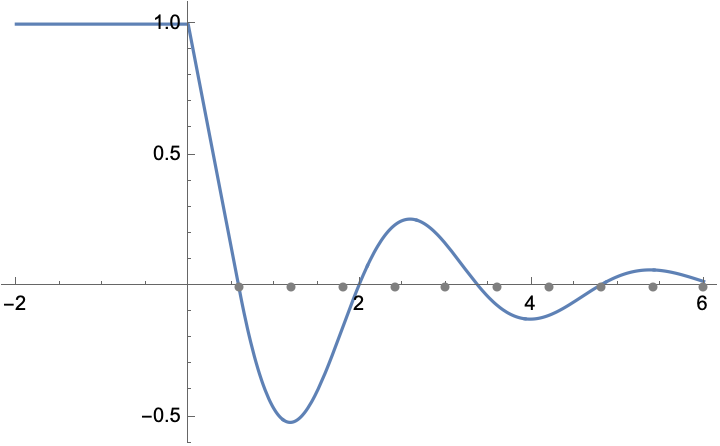
\includegraphics[width=.9\linewidth]{figures/simpledde.png}
      \caption{Solution to $\dot{x}(t) = -1.7x(t - 0.6)$}
      \label{fig:simpleddeimage}
    \end{subfigure}%
    \begin{subfigure}{.3\textwidth}
    %   \centering
      \begin{lstlisting}[basicstyle=\footnotesize]
        \\[Tau] := 0.6
        k := -1.7
        sol := NDSolve[
            {
                x'[t] == k*x[t - \[Tau]], 
                x[t /; t <= 0] == 1
            }, x, 
            { t, -5, 10*\[Tau] }
        ]
        Plot[
            Evaluate[x[t] /. sol], 
            {t, -2, 10*\[Tau]}
        ]
      \end{lstlisting}
      \caption{Mathematica Code}
      \label{fig:sub2}
    \end{subfigure}
    \caption{Numerically computed solution to \cref{eqn:ddesimpleoriginal}, in Mathematica}
    \label{fig:mathematicamagicsimple}
\end{figure}

\begin{remark}
    In the particular case that $k = -1, \tau = \frac{\pi}{2}$, we have \[
    \dot{x}(t) = -x(t - \frac{\pi}{2}),
    \]
    that is, the derivative of $x(t)$ is the negative of itself, phase shifted $\frac{\pi}{2}$. By inspection, its rather clear that the solution is simply \[
    x(t) = \cos t.    
    \]
\end{remark}

\subsection{Example 2 -  $\dot{x}(t) = rx(t)(1 - \frac{x(t-\tau)}{K})$}

The standard logistic equation, formulated by Verhulst, is of the form \begin{equation}
    \dot{x}(t)= rx(t)\left(1 - \frac{x(t)}{K}\right),
\end{equation}

where $r, K$ are strictly positive parameters. While rather simple, it provides enough analytical complexity to merit study \cite{strogatz}.

We consider now the modified, delayed form of this equation, formulated by Hutchinson \cite{Hutchinson}:
\begin{equation}\label{eqn:hutchinson}
    \dot{x}(t) = rx(t)\left(1 - \frac{x(t - \tau)}{K}\right).
\end{equation}

In the standard logistic equation, the "inner term" assumes that growth rate is relative to the current population, $x(t)$. Here, the inclusion of the delay term $\tau$ implies that the growth rate is relative to previous populations, indicating some type of "lag time" of effects \cite{ddesinglespecies}.

The method of steps could be used to find some solutions, but would be rather slow algebraically. As we are generally more interested with the dynamics of a system such as this rather than any potential analytic solution we could derive, we will, in this section, focus on more quantitative methods we may use to study DDEs, making sure to make comparisons with the study of ODEs.
\subsubsection{Steady States, Stability Analysis}

We can compute steady states of \cref{eqn:hutchinson} identically to "ordinary" dynamical systems:
\begin{align*}
    \dot{x}(t) = 0 &\iff rx(t)\left(1 - \frac{x(t - \tau)}{K}\right)\\
    &\iff x(t) = 0 \quad \vee \quad x(t - \tau) = K\\
    &\text{Let } x^*_1 \equiv 0, x^*_2 \equiv K
\end{align*}

Consider $x^*_1$. For small enough perturbations from the origin, $\dot{x} \approx rx(t)$ (neglecting the inner term; this is particularly "valid" if $K >> 0$). This has a simple exponential solution $x(t) = X_0 e^{rt}$, hence the origin is unstable as we have that $r >0$.

To analyze $x^*_2$, we first manipulate \cref{eqn:hutchinson}:
\begin{align*}
    \dot{x}(t) = rx(t)\left(1 - \frac{x(t - \tau)}{K}\right) &= \frac{r}{K}x(t)\left(K - x(t - \tau)\right)\\
    \tilde{x}(t) := x(t) - K \implies \dot{\tilde{x}}(t) &= \frac{r}{K}(\tilde{x}(t) + K)(-\tilde{x}(t - \tau))\\
    &= \underbrace{-\frac{r}{K}\tilde{x}(t)\tilde{x}(t - \tau)}_{\text{nonlinear}} \underbrace{- r \tilde{x}(t - \tau)}_{\text{linear}}
\end{align*}

Just as in ODE-based dynamical systems, we can perform linear stability analysis in a similar way even when delays are concerned. In this case, the LHS term involves both $\tilde{x}(t)$ and $\tilde{x}(t - \tau)$ and is thus nonlinear in $\tilde{x}$. Note that despite one of these terms not being "of the same time", this still results in a nonlinear term (this is particularly clear if $\tau = 0$). This gives a linearization \begin{equation}\label{eqn:linearization}
    \dot{\tilde{x}}(t) = -r \tilde{x}(t - \tau).
\end{equation}

This, again, looks like an exponential solution would fit, if the delay term were not present. To analyze this, we introduce the following extension of the characteristic polynomial to DDEs.

\subsubsection{Characteristic Equation, Bifurcation Analysis}

The \emph{characteristic equation} of a linear, homogenous \textit{ODE} of the form \[
0 = A_0y + A_1y' + \cdots + A_ny^{(n)}
\]
is a polynomial of the form \[
0 = A_0 + A_1r + \cdots + A_n r^n,
\]
whose roots $r_i$ allow us to find the general solution to $y$. This is derived from assuming a general complex exponential solution of the form $x(t) = x_0 e^{rt}$, which, when substituting into the original ODE, yield the characteristic equation.

Similarly, suppose we are working with a linear DDE of the form \[
\dot{x}(t) = A_0 x(t) + A_1x(t -\tau_1) + \cdots + A_n x(t - \tau_n).
\]
Assuming a solution of the form $x(t) = x_0e^{rt} \implies x(t - \tau_1) = x_0e^{r(t - \tau)}, \dots,$ then after substituting into the original DDE, we have \begin{align}
    re^{rt} = A_0e^{rt} + A_1e^{r(t - \tau_1)} + \cdots + A_n e^{r(t - \tau_n)},
\end{align}

which, after simplifications, gives the characteristic equation of linear DDEs:

\begin{equation}\label{eqn:characteristic}
    r = A_0 + A_1e^{-r\tau_1} + \cdots + A_ne^{-r\tau_n}.
\end{equation}
Note that $r \in \mathbb{C}$ by our assumptions, as previously.

We can then, as before, solve for the roots of this polynomial and find solutions. However, this is now a polynomial in terms of exponentials as well as a linear term, and thus presents far more challenges in solving analytically.

To see this, consider again \cref{eqn:linearization} from our example. In terms of our general formula \cref{eqn:characteristic}, we have $n = 1$, $A_0 = 0$ and $A_1 = -r$. Since we are already using $r$ as a parameter here, let $\lambda$ take the functional place of $r$ in the characteristic polynomial. Then, we have \begin{equation}\label{eqn:lambda}
    \lambda = -re^{-\lambda \tau}.
\end{equation}

To solve this equation, we adopt a standard approach; assume a complex solution, and simplify using Euler's formula until we can solve for real and imaginary solutions individually. Let $\lambda = \alpha + \beta i \in \mathbb{C} =\Re\lambda+ \Im\lambda i$. Substituting this into \cref{eqn:lambda}:
\begin{align*}
    \alpha + \beta i = -re^{-(\alpha + \beta i)\tau} &= -re^{-\alpha\tau}e^{-\beta\tau i}\\
    &= -re^{-\alpha \tau}\left[\cos\left(\beta \tau\right) - i \sin \left(\beta\tau \right)\right]\\
    &\implies \alpha +re^{-\alpha \tau} \cos (\beta \tau) = 0 \quad (i)\\
    &\implies \beta - re^{- \alpha \tau}\sin(\beta \tau) = 0\quad (ii)
\end{align*}

As in stability analysis of ODEs, linearized stability depends on the sign of the real part of $\lambda$; $\alpha$ positive indicates instability, while $\alpha$ negative indicates stability. Moreover, this means that the stability of the system will change when $\alpha = 0$, that is, when $\lambda$ is purely imaginary. Let $\beta_c, \tau_c$ be the values of the imaginary part of $\lambda$ and the delay at this critical value. This yields:
\begin{align*}
    &(i)\implies r \cos (\beta_c \tau_c) = 0\implies \beta_c\cdot \tau_c = \frac{\pi}{2} + 2\pi n, n \in \mathbb{N} \implies \tau_c = \frac{\pi}{2 \beta_c},\dots\\
    &(ii) \implies \beta_c = r \sin (\beta_c \tau_c) = \pm r \\
    &\hspace{12em}\implies \tau_c = \frac{\pi}{2 r} + \cdots \implies \beta_c = \pm r
\end{align*}

Moreover, when $\tau \in [0, \tau_c]$, $\alpha < 0$ (stable); if $\tau > \tau_c$, then $\alpha > 0$ (unstable). When $\tau = \tau_c$, note that $\beta$, the imaginary parts, are nonzero, which strongly implies the existence of a Hopf bifurcation at this point \cite{scientificcomputing}. Indeed, at this point, we have \[
\lambda = \alpha + \beta i = \pm r i,
\]
which gives a solution to \cref{eqn:linearization} of \begin{equation}
    \tilde{x}(t) = Ce^{t \lambda} = Ce^{\pm r i t} = C \cos (rt),
\end{equation}
where $C$ a constant determined by initial conditions. Recall that $\tilde{x} = x - K$, so we have, moreover, \begin{equation*}\label{eqn:solutionhopf}
    x(t) = C \cos (rt) + K.
\end{equation*}
Supposing an initial condition of $x(t \leq 0)$, then we would simply have \[
x(t) = (x(t \leq 0) - K) \cos (rt) + K.   
\]

This sinuisoidal solution supports our hasty bifurcation prediction, as we do indeed have periodic motion appearing from a steady state. Moreover, this periodic motion occurs between limit cycles occurring at $x(t \leq 0)$ and $x(t\leq 0) + 2K$, and hence centered about $x = x^*_2 = K$. This bifurcation is clear in the example solutions shown in \cref{fig:example2sol}, in which we include solutions plotted both in Cartesian coordinates $(x, y) \cong (t, x(t))$ and polar coordinates $(\theta, r) \cong (t, x(t))$ to better visualize the periodic behavior.

\begin{figure*}[!ht]
    \centering
    \includegraphics*[width=1.01\linewidth]{figures/example2.png}
    \vspace{1.5em}
    \caption{Solutions in (above) Cartesian and (below) polar to Hutchinson's Equation with initial value $x(t \leq 0) = 0.5, K = 1.2, r = 1.5$. From left to right, $\tau < \tau_c$ ($x_2^* = K$ stable), $\tau = \tau_c$ (Hopf bifurcation), and $\tau > \tau_c$ ($x_2^* = K$ unstable, period-2 limit cycle). }
    \label{fig:example2sol}
    \vspace{2em}
    \includegraphics*[width=\linewidth]{figures/example2polar.png}
\end{figure*}

We can also summarize this stability analysis in a bifurcation diagram, \cref{fig:bifurcationdiagramex2}, noting that, in this case, we keep the parameters $r, K$ constant, and we plot $x$ as a function of the time delay $\tau$.

\begin{figure*}[!ht]
    \centering
    \includegraphics*[width=0.4\linewidth]{figures/bifurcationdiagramexample2.png}
    \caption{Bifurcation diagram of Hutchinson's equation; $r = 1.5, K = 1.2$.}
    \label{fig:bifurcationdiagramex2}
\end{figure*}

Having thoroughly examined \cref{eqn:hutchinson}, we proceed to use the methods established as we turn our focus to climactic models.
\newpage

\section{Climactic Modelling - ENSO}

To discuss climactic modelling with DDEs, we will focus specifically on modeling the El Niño effect. Typically, trade winds in the Pacific, blowing west, bring warm water from South America towards Asia, which is then replaced by deep cold-water upwelling. \emph{El Niño} and \emph{La Niña}, collectively referred to as the \emph{El Niño-Southern Oscillation} (ENSO), are two well-studied climate phenomena which break this trend \cite{aboutelnino}. Despite efforts, a wholly comprehensive understanding of ENSO has yet to be fully achieved.

In general, from observational data, it is clear that ENSO is a periodically occurring event, though which varying periodicity and strength in effect. Moreover, it is clear that both atmospheric and oceanic conditions couple to, in some manner, alter ENSO \cite{climatedde}. In particular, it has been noticed that sea-surface temperature (SST) fluctuations are directly related to wave patterns in the Pacific. In this way, the application of a DDE model is very appropriate; some form of delay exists with regards to how a particular quantity is effected.

In the following sections, we will discuss several ENSO DDE models, their mathematical relevance to physical patterns, and briefly analyze their behavior.

\subsection{ENSO Model - Suarez}
\subsubsection{Physical Motivations}
One of the first DDE models for the ENSO effect was introduced by Suarez and Schopf in 1987 \cite{ensomodel}. The model is given as follows (modifying notation from the original text to more modern practices):
\begin{equation}\label{eqn:daoensomodel}
    \dot{h}(t) = h(t) - \left(h(t)\right)^3 - \alpha\cdot  h(t - \tau),
\end{equation}
in which $h$ represents anomaly of the \emph{thermocline depth}, $\alpha$ is a parameter value representing the scale of the delay term, and $\tau$ is the time delay (more specifically, $\tau$ in this model represents the wave transit time). The \emph{thermocline} refers to a layer of a body of water that divides the upper, surface layer (dubbed the "epipelagic zone") and the lower, cooler layer beneath (think of a nullcline, for the ocean)\cite{thermocline}. The epipelagic zone, being the upper layer, is where atmospheric conditions most directly influence oceanic conditions. In this way, the depth and strength of the thermocline is often studied as a direct proxy for SST \cite{randomnino}\cite{climatedde}. See \cref{fig:suarezschematic} for a more graphical, albeit simplified, view of the idea behind this model.

Here, the first, linear, non-delayed term represents an instantaneous feedback of the system, modeling a perturbation of the SST which hence heats the atmosphere. This effect is, physically, limited by various processes in both the ocean and atmosphere, a limit which is modeled by the polynomial, negative second term. Finally, the third term, the one that makes this a DDE in fact, represents the effect of oceanic waves (which, naturally, are delayed in their effect of a system). Here, $\alpha$ can be seen as a limiting parameter of this delay effect, and is taken as $\abs{\alpha} < 1$.

\begin{figure*}
    \centering
    \includegraphics*[width=0.7\linewidth]{figures/suarezmodel.png}
    \caption{Schematic behind the motivations of the Suarez model, based on the original schematic \cite{ensomodel}.}
    \label{fig:suarezschematic}
\end{figure*}

\subsubsection{Linear Stability Analysis}

Steady states occur at $\dot{h} = 0$:
\begin{align*}
    0 = h -h^3 - \alpha h(t - \tau)&\\
    &\implies h^*_0 = 0\\
    \implies h^2 = 1 - \alpha &\implies h^*_{1\pm} = \pm\sqrt{1 - \alpha} \iff \alpha < 1
\end{align*}

Linearized, \cref{eqn:daoensomodel} becomes \begin{equation}\label{eqn:linearizedsuarez}
    \dot{h}(t) = h(t) - \alpha h(t - \tau).
\end{equation}

We would like to investigate the stability of the solutions $h^*_1\pm$, the "outer", symmetrical steady states; physically, the $\pm$ can be interpreted as the system settling to a "cold" versus "warm" steady state \cite{ensomodel}. To investigate these, we can investigate perturbations about the steady state; let $h \mapsto h_1^* + \delta h$, taking $\delta$ to represent our "slight" perturbation. Substituting this into our original \cref{eqn:daoensomodel} yields
\begin{align*}
    \dot{\delta h}(t) = h_1^* + \delta h - (h_1^* + \delta h)^3 - \alpha (h_1^* + \delta h(t - \tau))\\
    = h_1^* + \delta h - (\delta h)^3 - 3 (\delta h)^2 h_1^* - 3 \delta h (h_1^*)^2 + (h_1^*)^3 - \alpha h_1^* - \alpha \delta h (t - \tau)
 \end{align*}
Ignoring higher order terms of $\delta h$ (ie those of $\order{(\delta h)^2}$):
\begin{align*}
    \dot{\delta h(t)} = (3 \alpha- 2)\delta h - \alpha \delta h(t - \tau).
\end{align*}
Seeking solutions to this (perturbed) DDE, we can utilize the \cref{eqn:characteristic} equation again (noting the similarities of this equation with \cref{eqn:hutchinson}):
\begin{equation}\label{eqn:squarezcharacter}
    r = 3 \alpha- 2 - \alpha e^{-r\tau}.
\end{equation}
Write $r = a + bi$. Then, we have \begin{align*}
    a + b i = 3 \alpha- 2 - \alpha e^{-a\tau}e^{-bi\tau} = 3 \alpha- 2 - \alpha e^{-a \tau}(\cos (b \tau) - i \sin (b \tau))\\
    \implies a = 3 \alpha- 2 - \alpha e^{-a \tau}\cos(b \tau) \quad (i), \qquad b = \alpha e^{-a \tau}\sin (b \tau) \quad (ii)
\end{align*}

Again, we can expect a bifurcation when $a$ changes sign, ie $a = 0$. This occurs:
\begin{align*}
    &(i) \implies 0 = 3\alpha -2 - \alpha \cos (b \tau) \implies b \tau = \arccos \left(\frac{3 \alpha-2}{\alpha}\right)\\
    &(ii) \implies b = \sin (b \tau) \implies \frac{1}{\tau} \arccos \left(\frac{3 \alpha-2}{\alpha}\right) = \sin( \arccos \left(\frac{3 \alpha-2}{\alpha}\right))=\sqrt{1 - \left(\frac{3 \alpha-2}{\alpha}\right)^2}\\
    &\hspace{12em}\implies \tau_c = \frac{\arccos \left(\frac{3-2 \alpha}{\alpha}\right)}{\sqrt{1 - \left(\frac{ 3 -2\alpha}{\alpha}\right)^2}}
\end{align*}

It is convenient to view this curve in $(\tau, \alpha)$ parameter space; see \cref{fig:squareparam}. For sufficiently small $\alpha$, the "choice" of $\tau$ is irrelevant; physically, this should make sense, as if $\alpha \ll 1$, then the delay term in \cref{eqn:daoensomodel} becomes negligible. Otherwise, we have two stability bifurcations that occur at the blue and orange curves for particular values of $\alpha, \tau$ for our steady state $h_1^*$. Note, moreover, as our solutions involves a $\arccos$ term, infinitely more curves exist to the right, for sufficiently large $\tau$.
\begin{figure*}[!ht]
    \centering
    \includegraphics*[width=0.55\linewidth]{figures/suarezparameter.png}
    \caption{Parameter space and neutral curves for \cref{eqn:daoensomodel} at $h_1^* = \pm\sqrt{1 - \alpha}$}
    \label{fig:squareparam}
\end{figure*}

Recall that this analysis has, so far, solely relied on the linearized model. We now turn to more numerical methods to confirm our linear stability analysis.

\subsubsection{Numerical Analysis}

\begin{figure*}[!ht]
    \centering
    \includegraphics*[width=0.8\linewidth]{figures/suareznumerics.png}
    \caption{
    Solutions $\dot{h}(t) = h(t) - h(t)^3 - \alpha h(t - \tau)$, with initial $h(t : t \leq 0) = h_1^*+0.1 = \sqrt{1 - \alpha}+0.1$. Parameters are taken as $\alpha = 0.7$, and (top left) $\tau = 1.75$, (top right) $\tau = 2.1$, (bottom left) $\tau = 5$, and (bottom right) $\tau = 10$. Dashed lines denote the location of the $\pm h_1^*$ steady states.
    }
    \label{fig:suareznumerics}
\end{figure*}

We use Mathematica to plot solutions to the Suarez model for varying $\tau$ and constant $\alpha$; see \cref{fig:suareznumerics}. With regards to stability changes, note that when $\tau = 1.75$, $h_1^*$ is stable, and is unstable when $\tau = 2.1$. In the previous section, our linearization predicted a change in stability when \[
    \tau_c = \frac{\arccos \left(\frac{3-2 \alpha}{\alpha}\right)}{\sqrt{1 - \left(\frac{ 3 -2\alpha}{\alpha}\right)^2}} \approx 1.44,
\]
that is, $\tau \approx 1.44$ when $\alpha = 0.7$ on the blue curve in \cref{fig:squareparam}. Numerically, this change in stability more closely occurs at $\tau \approx 2.0$. A "manually computed" bifurcation diagram can be seen in \cref{fig:suarezbfn}, where maxima and minima for the function were found for the solutions to $h(t)$ for varying $\tau$ over an interval of $[0, 10]$ for fixed $\alpha = 0.7$.
\begin{figure*}[!ht]
    \centering
    \includegraphics*[width=0.4\linewidth]{figures/suarezbfn.png}
    \caption{Bifurcation diagram for the Suarez model \cref{eqn:daoensomodel}.}
    \label{fig:suarezbfn}
\end{figure*}

More qualitatively, note the trends in behavior of $h$ as $\tau$ increases past this critical point; $h(t)$ becomes periodic, with amplitude staying relatively constant and period increasing. Moreover, rather large $\tau$ begin to approximate a square wave.


\subsection{Seasonal Forcing - Tziperman Model}

The previous model of SST perturbations, while mathematically nontrivial, made a lot of physical assumptions in order to include only one delay term. Tziperman et al \cite{tziperman} derived a model for thermocline depth including two delay terms, 
\begin{equation}\label{eqn:tzipermanog}
    \dot{h}(t) = \underbrace{a A (\kappa, h (t - \tau_p))}_{p} \underbrace{- b A ( \kappa, h (t - \tau_n))}_{n} + c \cos (2 \pi t), \quad A (\kappa, h) = \begin{cases}
        d_u \tanh \left(\frac{\kappa}{d_u}h\right) & h \geq 0\\
        d_l \tanh \left(
            \frac{\kappa}{d_l}h
        \right) & h < 0
    \end{cases}
\end{equation}


\subsubsection{Physical Motivations}


In \cref{eqn:tzipermanog}, $\tau_p$ and $\tau_n$ are fixed delay times, corresponding to their respective positive ($p$) and negative ($n$) feedback terms; $a$ and $b$
are positive constants. The function $A(\kappa, h)$ serves as a coupling function between the atmosphere and ocean effects  \cite{coupling}; $d_h > 0$ and $d_l < 0$. 

Moreover, the $p$ term attempts to model the effect of a \emph{Kelvin wave} and the $n$ term that of a \emph{Rossby wave}. A \emph{Rossby} or \emph{planetary} wave is one that arises as a result of the varying effect of the Coriolis effect as a function of latitude (that is, it is directly related to the Coriolis parameter, which itself relies on latitude)\cite{fundamentalsatmo} \cite{naoorossby}.
\begin{remark}
    Rossby waves can be rigorously mathematically described \cite{fundamentalsatmo}, but this is beyond the scope of this paper; for our purposes, it suffices to understand that Rossby waves are large, slow-moving oceanic movements that have clear physical associations with thermocline depth.
\end{remark}
\emph{Kelvin} waves arise as a result of rising SST; greater SST in the west leads results in a long-distance wave traveling east \cite{climatedde}.

Together, Kelvin and Rossby waves describe a feedback loop which is well-studied in the context of El Niño and general atmospheric conditions; their delayed effect (taking around scale 1-6 months to complete their feedback loops across the Pacific \cite{climatedde}) are well suited to modeling via DDEs.

The final term of \cref{eqn:tzipermanog}, $c \cos (2 \pi t)$, represents a seasonal forcing term; here, time $t$ is scaled such that the period of the seasonal effect is $2 \pi$ (ie, $\cos (2\pi \cdot 0) = \cos (2 \pi \cdot 1)$).

\subsubsection{Numerical Analysis}

For ease of analysis, we will primarily consider a simplified version of \cref{eqn:tzipermanog}, where $a = 0, d_u = 1, d_l = -1$, and hence we have only the parameters $b$ (related to the effect of Rossby waves), $\kappa$ (related to the atmosphere-ocean coupling), and $c$ (related to the effect of the seasonal forcing), as well as the time delay $\tau_n$ (which we will now call $\tau$ for concision) \cite{ghil}.
\begin{equation}\label{eqn:simplifiedtz}
    \dot{h}(t) = -b \tanh (\kappa h (t - \tau)) + c \cos (2 \pi t).
\end{equation} 

Note that, unlike any other models we have analyzed so far, this DDE has an explicit time dependence in the rightmost term. This goes away if $c = 0$, which results in a fairly trivial model with a single steady state at $h = 0$, which is always stable. The $\tau$ term does lead to oscillations about the steady state before settling down, but in the long term solutions will always go to zero.

The model, in full, is quite difficult to analyze analytically. Instead, we will investigate different parameter values, and describe behaviors more qualitatively in context of climactic conditions. Specifically, while in previous models we focused primarily on the effects of time delay with fixed parameters, we will be instead focusing on relatively constant $\tau \approx 0.5$ (we are working on the time scale of years) and observing changes due to $\kappa$.

\noindent\textbf{El Niño: } numerically solving \cref{eqn:simplifiedtz} with parameters of $\kappa = 5, \tau = 0.65, c = 1, b = 1.5$ results in a periodic, albeit of irregular amplitude, behavior as can be seen in \cref{fig:elnino}. The relatively low value of $\kappa$ indicates relatively low coupling of the ocean and atmosphere, as is understood to be the case in a regularly temperate El Niño effect. Interpreting $h(t)$, roughly, as average temperature, this plot corresponds to fairly normal, primarily seasonal climate effects. 
\newline
\begin{figure*}
    \centering
    \includegraphics*[width=0.8\textwidth]{figures/nino.png}
    \caption{(Left) El Niño: $\kappa = 5, \tau = 0.65, c = 1, b = 1.5$. (Right) La Niña: $\kappa = 50, \tau = 0.42, c = 1, b = 1.5$.}
    \label{fig:elnino}
\end{figure*}

\noindent\textbf{La Niña: } by contrast, taking parameters of $\kappa = 50, \tau = 0.42, c = 1, b = 1.5$, we can see solutions to \cref{eqn:simplifiedtz} more physically representative of a La Niña effect. A higher atmosphere-ocean coupling parameter $\kappa$ leads to more irregular heating. The high peaks represent irregular bouts of higher temperatures, indicative of a La Niña pattern.
\newline

\noindent\textbf{High Coupling: } a natural question, seeing the previous situations, is what does the extreme (large $\kappa$) of the ocean-atmosphere coupling look like? In this case, the $\tanh$ component of the model essentially becomes a step function, and dynamics would hence be more determined by the constant $b$ parameter rather than the delay term. This results in much more unique behavior than the previous two cases, as is evident in \cref{fig:weird}. In these cases, we maintain the same periodic behavior, but now with slight, yet rapid, perturbations that occur near the midpoint of each wavelength. Both the amplitudes and durations of these perturbations are proportional to the given value of $b$.

Physically, these effects have been interpreted as representing \emph{Westerly Wind Bursts} or \emph{Madden-Julian oscillations}\cite{wwb}, major fluctuations in regular climactic conditions reminiscent of the behavior visible here.
\begin{figure*}
    \centering
    \includegraphics*[width=1\linewidth]{figures/weird.png}
    \caption{(High Coupling) $\kappa = 500, \tau = 0.005, c = 1$; left to right: $b = 0.75, 1, 1.25$.}
    \label{fig:weird}
\end{figure*}

In all, the models we have investigated have all, despite their simplicity and the physical assumptions they inherently contain, demonstrate highly complex behaviors. While they only scratch the surface of what DDEs are capable of modeling in the context of climatology, they nonetheless demonstrate the high potential of these types of models, and moreover, the techniques we may use to analyze them.

\section{Conclusion}

In this paper, we explored general analytical and computational techniques to approach DDEs, with a focus on relatively simple examples used in climate modelling. In general, DDEs provide a way to mathematically model complex natural systems, particularly those that involve some sort of intrinsic feedback or more simply delay mechanism. DDEs, specifically in the context of more applied practices, are still relatively underdeveloped in their theory. Nevertheless, given their practical similarity to ODEs and their more general applicability, they are certainly valuable tools worth further study.


$$\blacklozenge$$


\begin{remark}
    All plots, diagrams, and code listings, unless otherwise cited, are of my own creation. Source code, written in Mathematica, is posted \href{https://github.com/louismeunier/math376-final}{here}.
\end{remark}
\printbibliography
\end{document}
